\section{ARM Cortex}
\subsection{Overview}
\begin{frame}
    \frametitle{ARM}
    \framesubtitle{Overview}
    ARM Cortex
    \begin{itemize}
        \item \textbf{A}dvanced \textbf{R}ISC \textbf{M}achines
        \item sell License
        \item up to 64bit
    \end{itemize}
    \begin{block}{ARM Today}
		The Apple A8 is built up of a 64-Bit-ARM-CPU
    \end{block}
\end{frame}

\subsection{Families}
\begin{frame}
    \frametitle{ARM}
    \framesubtitle{Families}
   ARM Cortex Families:
    \begin{itemize}
        \item A: Application
        \item R: Realtime
        \item \textbf{M: Microcontroller}
    \end{itemize}
    \begin{block}{Instruction Set}
       M0,\textbf{ M0+}, M1 $<$  M3 $<$  \textbf{M4} $<$ M4 FPU
    \end{block}
\end{frame}

\subsection{Instruction set}
\begin{frame}
    \frametitle{ARM}
    \framesubtitle{Instruction set}
    \begin{figure}
        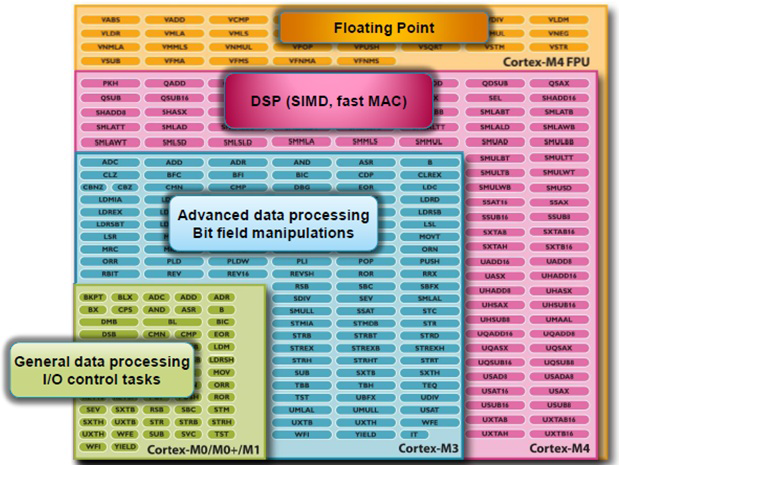
\includegraphics[width=0.8\textwidth]			{fig/instructionset.png}
        \caption{Instruction set}
    \end{figure}
\end{frame}

\subsection{Interrupts}
\begin{frame}
    \frametitle{ARM}
    \framesubtitle{Interrupts}
    16 predefined Interrupts
    Priorities
        \begin{itemize}
        \item 8bit Priority Register
        \item FSL M0+: 2bits = 4 Priorities
        \item FSL M4 : 4bits = 16 Prio
    \end{itemize}
    \begin{block}{Reihenfolge Priorities}
        the lower the prio or subprio number - the higher prio!
    \end{block}
\end{frame}
